\documentclass{standalone}

\usepackage{tikz}

\begin{document}
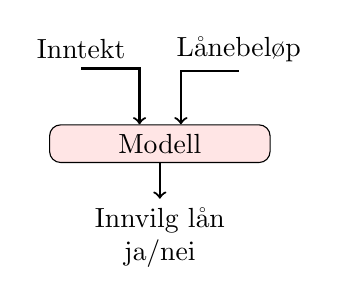
\begin{tikzpicture}
   \tikzstyle{every node}=[node distance=12mm]

   \node (ml) [draw,rounded corners,fill=red!10,minimum width=28mm] {Modell} ;
   \node (i1) [above of=ml,xshift=-10mm] {Inntekt} ;
   \node (i2) [above of=ml,xshift=10mm] {Lånebeløp} ;

   \draw [thick,->] (i1.south) -| ([xshift=-10mm]ml) ;
   \draw [thick,->] (i2.south) -| ([xshift=10mm]ml) ;

   \node (dec) [below of=ml] {\parbox{20mm}{\centering Innvilg lån\\ja/nei}} ;

   \draw [thick,->] (ml) -- (dec) ;

\end{tikzpicture}
\end{document}
